
\subsubsection{Задача $topN$}
Схема решения задачи $topN$ заключается в построении кластера соседей
$\nut = \{u: u_a \ru u\}$ активного пользователя $u_a$, который выступает в
роли центра кластера. После того, как кластер был
построен, выбирается $N$ объектов, которые близки для большинства
пользователей.

Это решение основано на правиле вывода $\Pi_C$ --- пусть объект $i$ близок
для большинства пользователей кластера $\nut$: $(\frac{1}{|\nut|} \sum \limits_{u \in
\nut} \rho(u,i)) \ge \Delta_{\R}$, а функциональная зависимость $f_p$
прогнозной функции $\rh$ определяется средним значением оценок близостей
соседей $\rho(u,i)$. Тогда $\rh(u_a, i) = f_p(\{\rho(u, i)\})
> \Delta_{\R}$, и тогда можно утверждать, что $u_a \R i$. $N$ таких объектов
составляет решение задачи $topN$.

Опишем возможную\footnote{Модели могут отличаться такими параметрами, как,
например, функция $\du$, поэтому нижеописанная модель является одной из
возможных}
модель CОМ
\footnote{
	На данном этапе без оценки качества $\mathcal{E}_{topN}$
	}
 и на ее примере решим
задачу $topN$  \cite{amazon-linden}.%TODO: set cite

\begin{itemize}
	\item $c_X(u_a) = (x_1, x_2, ..., x_n)$
\begin{equation*}
  x_i =
  \begin{cases}
	1, &\text{если $u_a \R i$}\\
	  0, &\text{иначе}
  \end{cases}
\end{equation*}
	Это распространенный способ представления контента,
	где координаты соответствуют объектам
		 \cite{topn1}.
	Данный способ представления
	информации о пользователях заимствован из информационного поиска
	 \cite{e-commerce,empirical-cf,ir4};
	\item $c_Y$ не определяется, так как с объектами в СОМ работа не проводится;
	\item $\di(u_a,u) =\cos(\angle(c_X(u_a),c_X(u)))$.
\end{itemize}

Чтобы сформировать кластер соседей, производится линейный поиск соседей
на множестве пользователей \cite{amazon-item2item}. Для построения результирующего
множества просуммируем контенты (данная операция
допустима, так как контент представляет из себя вектор) соседей,
и выберем те координаты $i$, которые обладают наибольшими значениями
и $(i, \rho(u_a,i)) \not \in P_0$.


На рисунке (\ref{dia:nut}) изображена блок-схема алгоритма
построения кластера соседей $\nut$, которой соответствует псевдокод
, представленный на изображении <<Построение множества соседей для активного
		пользователя $u_a$ при решении задачи $topN$>>
(\ref{alg:nut}).
\begin{figure}[htb]
	\caption{Блок-схема алгоритма построения кластера $\nut$}
\begin{center}
	\label{dia:nut}
 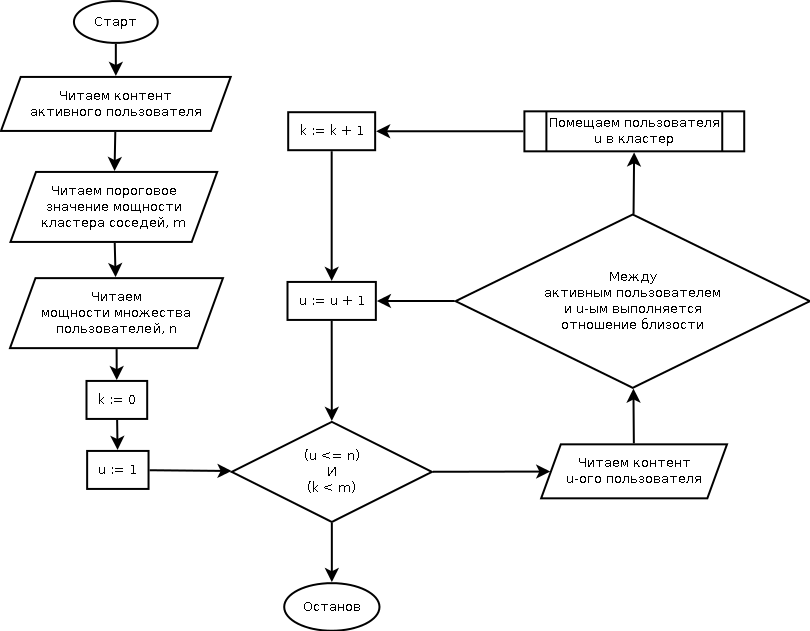
\includegraphics[width=7in,height=8in]{pics/algs/nut.png}
\end{center}
\end{figure}

\begin{figure}[htbp]
	%\begin{algorithm}
		\caption{Построение множества соседей для активного
		пользователя $u_a$ при решении задачи $topN$}
		\label{alg:nut}
		\begin{algorithmic}[1]
			\State $\nut \gets \varnothing$
			\State $k \gets 0$
			\For {$u \gets 1 \to |U|$}
			\If{$u_a \ru u$}
			\State $\nut \gets \nut \bigcup \{ u \}$
			\State $k \gets k + 1$
			\EndIf
			\If{$k > M$}\Comment{Ограничение на размер множества соседей}
			\State Стоп
			\EndIf
			\EndFor
		\end{algorithmic}
	%\end{algorithm}
\end{figure}


На рисунке (\ref{dia:topn-srs}) изображена блок-схема решения задачи $topN$ в
$COM$, которой соответствует псевдокод, представленный на изображении <<Стандартный алгоритм решения задачи $topN$>>  (\ref{alg:topn-srs}).
\begin{figure}[htb]
	\caption{Решение задачи $topN$ в $COM$}
	\begin{center}
		\label{dia:topn-srs}
		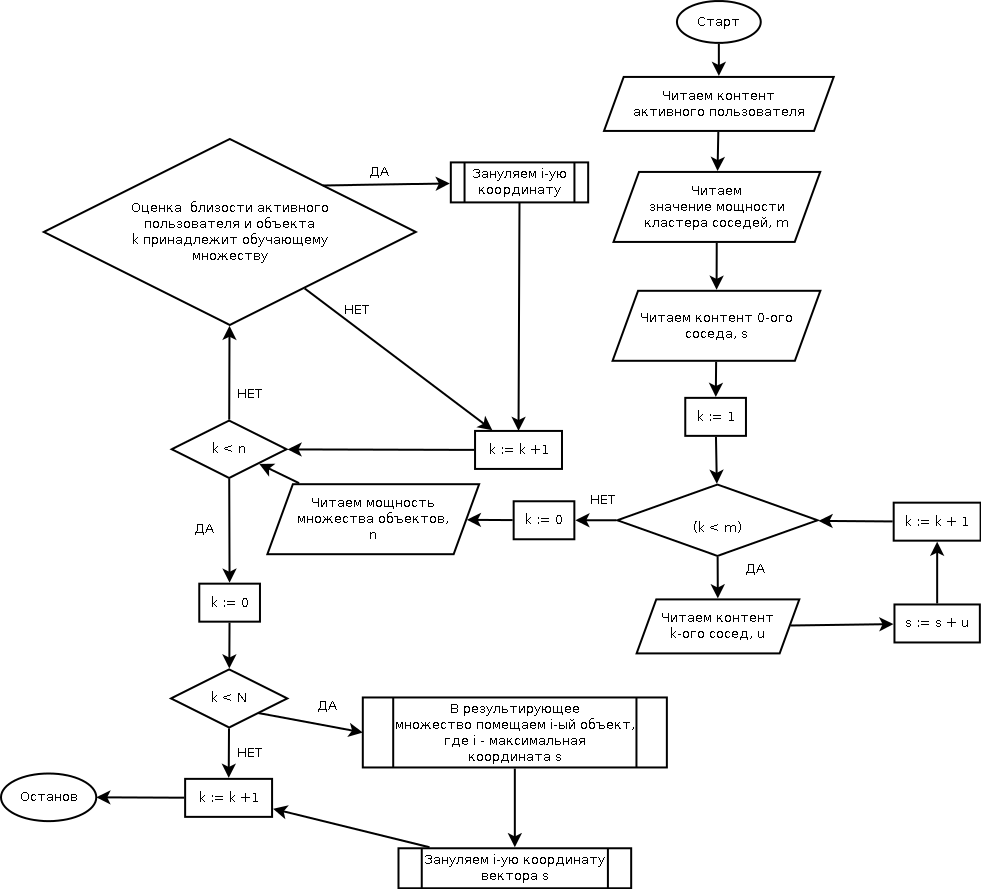
\includegraphics[width=7in,height=8in]{pics/algs/topn-srs.png}
	\end{center}
\end{figure}

\begin{figure}[htbp]
	%\begin{algorithm}
		\caption{Стандартный алгоритм решения задачи $topN$}
		\label{alg:topn-srs}
		\begin{algorithmic}[1]
			\State $s \gets \sum \limits_{u \in \nut} u$ \Comment{Вектор-сумма}
			\For {$i \gets 1, i \le |I|$}
			\If {$\exists \rho(u_a,i)$} \Comment{Если активный пользователь уже оценил
			объект, то он должен отсутствовать в результирующем множестве}
			\State $s_i \gets 0$ \Comment{Зануляем $i$-ую координату}
			\EndIf
			\EndFor
			\State $\overline{P}^a_{\bot} \gets \varnothing$
			\State $I_{topN} \gets \varnothing$
			\For {$k \gets 1, k \le N$}
			\State $i \gets \underset{i} {\mathrm{\max}}$ $s$
			\State $I_{topN} \gets I_{topN} \bigcup \{i\}$
			\State $\overline{P}^a_{\bot} \gets \overline{P}^a_{\bot} \bigcup
			\{ 0 \}$ \Comment{Для решения задачи нужно составить множество объектов, а не
			определить близость, поэтому $\rho(a,i)=0$, так как тогда $\forall
			\epsilon_0:$ $u_a \R i$}
			\State $s_i \gets 0$
			\State $k \gets k + 1$
			\EndFor
		\end{algorithmic}
	%\end{algorithm}
\end{figure}
